\documentclass[11pt]{article}

\usepackage{amssymb}
\usepackage{amsmath}
\usepackage{esint}
\usepackage{setspace}
\usepackage{graphicx}
\usepackage{subfig}
\usepackage{color}
\usepackage[left=1.2in, right=1in, top=1in, bottom=1in]{geometry}
\usepackage{verbatim}
\usepackage{hyperref}

\begin{document}

\section{Introduction}

A common claim regarding flight, and lift generation in particular, is that
Newton's laws of motion require the lift to be equal to the rate of change of
downward momentum of the surrounding air. In this analysis, Newton's laws of
motion are methodically applied to a volume of air surrounding a wing to show
the actual relationship between lift and the rate of change of momentum of the
air. These relationships are then explored numerically using an inviscid panel
code. The analysis shows that in general, lift is not equal to the rate of
change of downward momentum, even for an isolated wing in free air.

\section{Rate of Change of Momentum}\label{sec:momchange}

The rate of change of momentum in a differential (infinitesimal) element of
fluid with mass $dm$ is given by the substantial derivative:

\begin{equation}
\frac{D(\vec{V}dm)}{\partial t} = \frac{\partial(\vec{V}dm)}{\partial t}
                                 + \vec{V}\cdot\vec{\nabla}\vec{V}dm,
\end{equation}

\noindent where $\vec{V}$ is the fluid velocity vector and $\vec{\nabla}$ is the
gradient operator. Using an Eulerian tracking of the fluid element, the
differential volume, $dV$, of the element remains constant while the density,
$\rho$, may vary. Therefore,

\begin{equation}
\frac{D(\rho\vec{V}dV)}{\partial t} = \frac{\partial(\rho\vec{V}dV)}{\partial t}
                                    + \vec{V}\cdot\vec{\nabla}\rho\vec{V}dV.
\label{eq:substantial}
\end{equation}

We are interested in the rate of change of momentum of a large fluid volume due
to the presence of a lifting body, so we integrate Eq. \ref{eq:substantial} over
a large volume $V$:

\begin{equation}
\iiint_V\frac{D(\rho\vec{V})}{\partial t}dV = 
\iiint_V\frac{\partial(\rho\vec{V})}{\partial t}dV +
\iiint_V\vec{V}\cdot\vec{\nabla}\rho\vec{V}dV.
\label{eq:total_momchange}
\end{equation}

Equation \ref{eq:total_momchange} represents the total rate of change of
momentum of the fluid in $V$. The last term in the equation can
be converted from a volume integral to a surface integral using the divergence
theorem as follows:

\begin{equation}
\iiint_V\vec{V}\cdot\vec{\nabla}\rho\vec{V}dV = 
\iiint_V\rho\vec{V}\vec{\nabla}\cdot\vec{V}dV = 
\oiint_S\rho\vec{V}(\vec{V}\cdot\hat{n})dS,
\label{eq:divergence}
\end{equation}

\noindent where $S$ represents all bounding surfaces of volume $V$, $\hat{n}$
is the vector normal to the surface on $S$, and $dS$ is an infinitesimal element
of area on $S$. The bounding surfaces include:

\begin{itemize}
  \item The outer surfaces of the volume (e.g., a bounding box or sphere), and
  \item any interior surfaces, such as the surfaces of a wing or aircraft.
\end{itemize}

Substituting Eq. \ref{eq:divergence} into Eq. \ref{eq:total_momchange},

\begin{equation}
\iiint_V\frac{D(\rho\vec{V})}{\partial t}dV = 
\iiint_V\frac{\partial(\rho\vec{V})}{\partial t}dV +
\oiint_S\rho\vec{V}(\vec{V}\cdot\hat{n})dS.
\end{equation}

\noindent If the flow is at steady state, then the first term on the right-hand
side of the equation is 0, so

\begin{equation}
\iiint_V\frac{D(\rho\vec{V})}{\partial t}dV = 
\oiint_S\rho\vec{V}(\vec{V}\cdot\hat{n})dS.
\label{eq:momrate}
\end{equation}

\section{Newton's Second Law}

Newton's Second Law of motion states that the sum of all forces on an object is
equal to its rate of change of momentum. Applied to the fluid in the volume $V$
at steady state, using the result of Section \ref{sec:momchange}, this law is
expressed by the following equation:

\begin{equation}
\oiint_S\rho\vec{V}(\vec{V}\cdot\hat{n})dS = \sum{F},
\end{equation}

\noindent where $\sum\vec{F}$ is the vector sum of forces acting on the fluid
inside the volume $V$. The next step is to write an expression for
$\sum{\vec{F}}$.
Assuming an inviscid flow with negligible body forces acting on the fluid, all
forces are produced by pressure acting on the boundaries. Therefore,

\begin{equation}
\oiint_S\rho\vec{V}(\vec{V}\cdot\hat{n})dS = -\oiint_Sp\hat{n}dS.
\label{eq:2nd_law1}
\end{equation}

\noindent The negative sign in front of the pressure term is due to the fact
that pressure pushes inward on the fluid from the bounding surface while
$\hat{n}$ points outward. In cases where there are both an inner surface $S_i$
and an outer surface $S_o$, it is convenient to divide the integral into two
separate integrals, one over $S_i$ and another over $S_o$. Applying that
approach to Eq. \ref{eq:2nd_law1},

\begin{equation}
\oiint_{S_o}\rho\vec{V}(\vec{V}\cdot\hat{n})dS +
\oiint_{S_i}\rho\vec{V}(\vec{V}\cdot\hat{n})dS =
-\oiint_{S_o}p\hat{n}dS - \oiint_{S_i}p\hat{n}dS.
\label{eq:2nd_law2}
\end{equation}

The last term in the equation represents the pressure force acting on the fluid
due to the inner surfaces. In the case of a wing or aircraft in steady flight,
this is the force applied to the fluid by the wing or aircraft. Applying
Newton's Third Law of motion,

\begin{equation}
\oiint_{S_o}\rho\vec{V}(\vec{V}\cdot\hat{n})dS +
\oiint_{S_i}\rho\vec{V}(\vec{V}\cdot\hat{n})dS =
-\oiint_{S_o}p\hat{n}dS - \vec{F_A},
\label{eq:2nd_law3}
\end{equation}

\noindent where $\vec{F_A}$ is the aerodynamic force acting on the aircraft,
made up of lift and induced drag.
Because the inner surfaces are solid walls, no fluid can pass through them,
implying that $\vec{V}\cdot\hat{n}$ in the second term of Eq. \ref{eq:2nd_law3}
must be 0, and thus the entire term drops out of the equation. Therefore, the
aerodynamic force on the aircraft is related to
the rate of change of momentum of fluid in the volume (the first term in
Eq. \ref{eq:2nd_law3}) and the pressure force on the outer boundaries (the
first term on the right-hand side in Eq. \ref{eq:2nd_law3}) as follows:

\begin{equation}
\vec{F_A} = -\oiint_{S_o}\rho\vec{V}(\vec{V}\cdot\hat{n})dS
          - \oiint_{S_o}p\hat{n}dS.
\label{eq:2nd_law4}
\end{equation}

If the coordinate system is chosen so that $\alpha$ is the angle between the
freestream flow direction and the x-axis, then lift and induced drag are as
follows:

\begin{equation}
L = \left[-\oiint_{S_o}\rho\vec{V}(\vec{V}\cdot\hat{n})dS -
           \oiint_{S_o}p\hat{n}dS\right]
    \cdot(-\sin\alpha\hat{i} + \cos\alpha\hat{k})
\label{eq:lift}
\end{equation}

\begin{equation}
D_i = \left[-\oiint_{S_o}\rho\vec{V}(\vec{V}\cdot\hat{n})dS -
             \oiint_{S_o}p\hat{n}dS\right]
      \cdot(\cos\alpha\hat{i} + \sin\alpha\hat{k}).
\label{eq:induced_drag}
\end{equation}

Consider the first term in brackets on the right-hand side of Eq. \ref{eq:lift}.
This is the rate of change of momentum of the fluid. The second term in
brackets is the pressure force on the outer boundaries, which was not accounted
for at all in the claim presented in the introduction. Therefore, this equation
shows immediately that the claim in the introduction can only be true if the
pressure term goes to 0 in the limit as the volume of air considered becomes
infinitely large. In other words, perhaps when \textit{all} the air
accelerated by the wing is accounted for, the lift is in fact equal to the rate
of change of downward momentum of the air. This possibility will be examined
numerically for a wing in steady, inviscid flow in the following sections.

\section{Numerical Method}

LORAAX, a panel code based on potential flow with corrections for
compressibility, a coupled quasi-2D integral boundary layer method for viscous
effects, and wake roll-up, is used to compute the flow solution. In accordance
with the assumptions of the present analysis, the code is run in inviscid mode
(boundary layer
calculations disabled) and with a static, planar wake. For the sake of
simplicity, the Mach number is 0.025 -- well within ``incompressible'' range --
though compressibility corrections are
still active and density is not assumed constant. The  theory of the fluid
solver is out of the scope of this paper, but it has been validated against both
experimental data and solutions from higher-fidelity CFD solvers.

In the present analysis, the inner fluid boundary is
a rectangular wing with an aspect ratio of 8 and a symmetrical NACA 0012
airfoil. The outer boundary is represented by a box with faces aligned with the
coordinate axes. As part of the analysis, different sizes and shapes of outer
boxes are evaluated, and the size of rectangular panels making up each face is
varied. Figure \ref{fig:domain} illustrates the fluid domain. In this example,
the fluid volume is a cube with side length 2.5 times
the wingspan and a 10x10 grid to discretize each face of the outer box.

\begin{figure}
\centering
  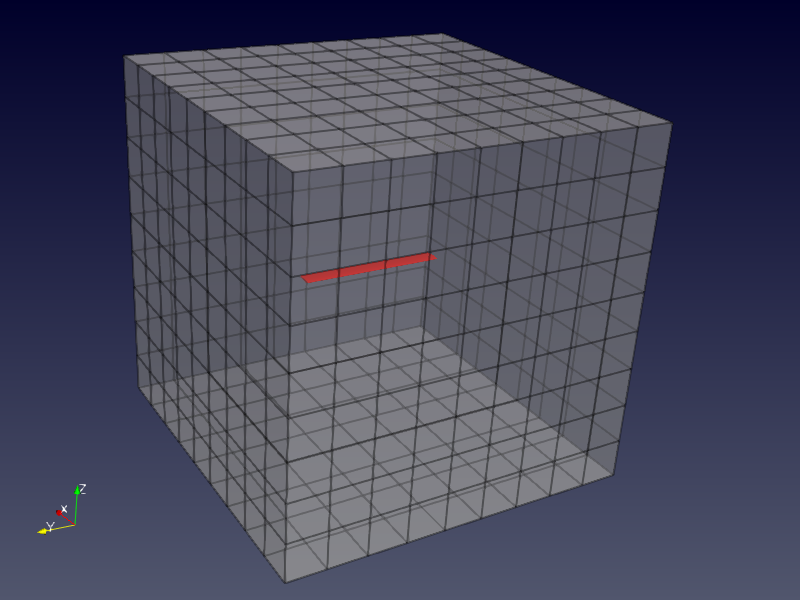
\includegraphics[width=0.75\textwidth]{images/domain.png}
\caption{Wing (red) inside a cubic fluid domain.}
\label{fig:domain}
\end{figure}

The rate of change of momentum in the volume is evaluated numerically by
discretizing Eq.
\ref{eq:momrate}. Let the area of the $i^\text{th}$ rectangular panel on the
outer box be $\Delta S_i$, the outward-pointing normal vector $\hat{n}_i$, and
the local density and velocity $\rho_i$ and $\vec{V}_i$, respectively. Let $N$
be the total number of rectangular panels on the outer box. The rate of change
of momentum in the fluid volume becomes

\begin{equation}
\iiint_V\frac{D(\rho\vec{V})}{\partial t}dV \approx 
\sum_{i=1}^N \rho_i\vec{V}_i\cdot\hat{n}_i\Delta S_i.
\label{eq:momrate_numerical}
\end{equation}

The left and right side are only approximately equal because the discretization
process introduces numerical error. However, as $\Delta S$ becomes smaller and
smaller, the numerical error also becomes smaller, eventually vanishing in the
limit as $\Delta S \rightarrow 0$. Though it is not possible in practice for
$\Delta S$ to be vanishingly small, it can be small enough that the error
becomes negligible. When this condition is met, the numerical solution is called
\textit{grid-converged}, and for practical purposes the left and right sides in
Eq. \ref{eq:momrate_numerical} become equal. In the following numerical
approximations, it is assumed that the solution is grid-converged, and the
equal sign is used.

The lift and induced drag are computed numerically as follows:

\begin{equation}
L = \left[-\sum_{i=1}^N\rho_i\vec{V}_i(\vec{V}_i\cdot\hat{n}_i)\Delta S_i -
           \sum_{i=1}^N p_i\hat{n}_i\Delta S_i\right]
    \cdot(-\sin\alpha\hat{i} + \cos\alpha\hat{k})
\label{eq:lift_numerical}
\end{equation}

\begin{equation}
D_i= \left[-\sum_{i=1}^N\rho_i\vec{V}_i(\vec{V}_i\cdot\hat{n}_i)\Delta S_i -
           \sum_{i=1}^N p_i\hat{n}_i\Delta S_i\right]
      \cdot(\cos\alpha\hat{i} + \sin\alpha\hat{k}),
\label{eq:induced_drag_numerical}
\end{equation}

\noindent where $\hat{i}$ and $\hat{k}$ are unit vectors in the $x$ and $z$
directions, respectively.
LORAAX also computes lift and induced drag using Trefftz plane analysis, and the
results of Eqs. \ref{eq:lift_numerical} and \ref{eq:induced_drag_numerical} can
be compared with the Trefftz-plane result to verify that the method has been
implemented correctly and to evaluate grid convergence. The component of rate of
change of fluid momentum in the direction opposing lift (the rate of change of
``downward'' momentum) in the volume $V$ is

\begin{equation}
\frac{D(m\vec{V})_\text{down}}{\partial t} = 
-\sum_{i=1}^N \rho_i\vec{V}_i\cdot\hat{n}_i\Delta S_i
\cdot(-\sin\alpha\hat{i} + \cos\alpha\hat{k}).
\label{eq:downward_momrate}
\end{equation}

\subsection{Grid Convergence}\label{sec:grid_convergence}

Before determining the number or size of panels in the farfield to accurately
resolve the rate of change of momentum inside the volume, grid convergence of
the flow solution itself needs to be evaluated. Figure \ref{fig:solver_convergence}
depicts the lift and induced drag coefficients for a rectangular NACA 0012 wing
with $AR = 8$, Mach = 0.025, and $\alpha = 5^\circ$ with different numbers of
panels placed on the surface.
These force coefficients have been computed using the Trefftz plane method.
The coarsest wing evaluated had 20 panels in the chordwise direction, on both
the top and bottom surfaces (40 total), and 20 in the spanwise direction, for
440 total degrees of freedom in the solution. The finest had 99 panels in the
chordwise direction and 90 in the spanwise direction, for 8,910 total degrees
of freedom. Each wing had panels clustered closer together near the leading
and trailing edges and the wingtips.

\begin{figure}
\centering
  \subfloat[Lift coefficient]{
    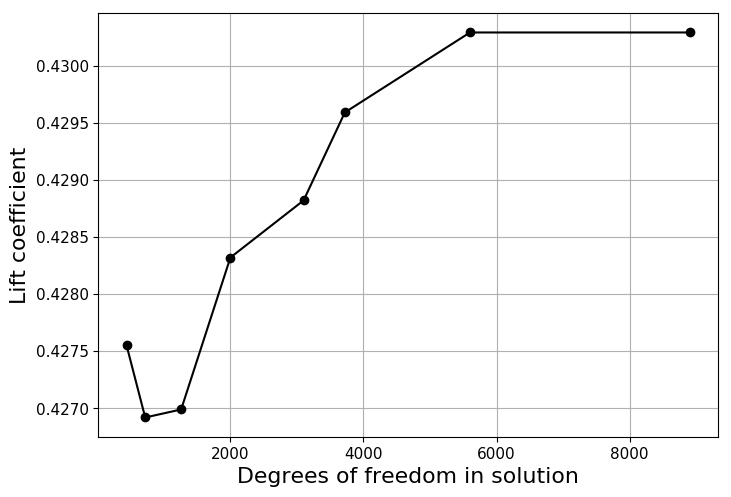
\includegraphics[width=0.49\textwidth]{images/lift_convergence.png}}
  \subfloat[Drag coefficient]{
    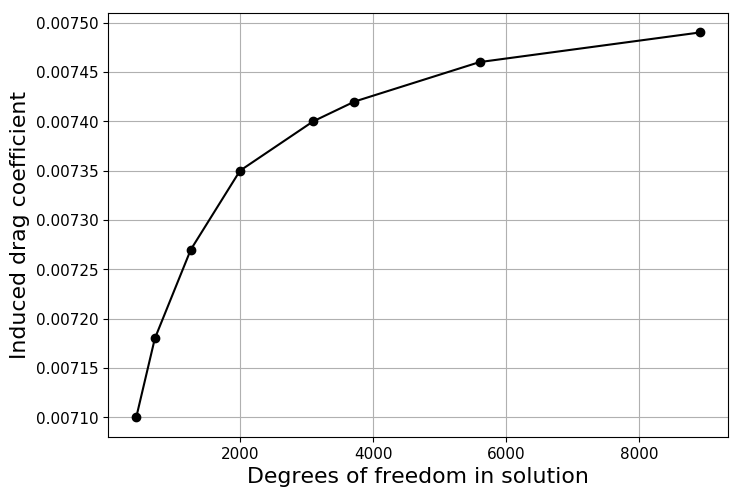
\includegraphics[width=0.49\textwidth]{images/drag_convergence.png}}
\caption{Flow solver grid convergence.}
\label{fig:solver_convergence}
\end{figure}

\begin{figure}
\centering
  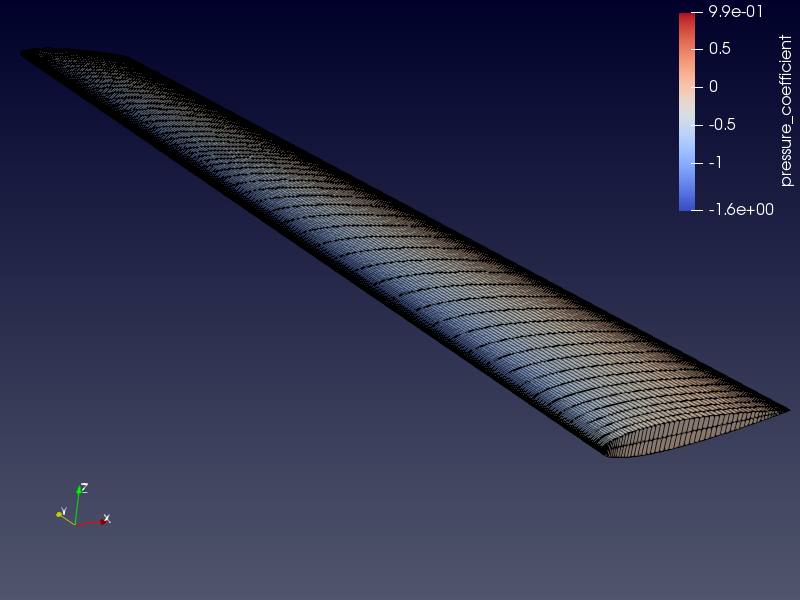
\includegraphics[width=0.60\textwidth]{images/61x31_wing.png}
\caption{NACA 0012 wing with $AR=8$ and 3,720 degrees of freedom.}
\label{fig:61x31_wing}
\end{figure}

Figure \ref{fig:solver_convergence} demonstrates that both lift and induced drag
approach a single result as the surface grid is refined. The induced drag
approaches the grid-converged result asymptotically, while the lift is not as
smooth. However, even the coarsest grid produces a lift coefficient that
differs from the finest grid by less than 1\%, while induced drag is more
sensitive to grid resolution. Though any of these grids should work well for
evaluating lift, the third-finest grid has been selected as the preferred choice
due to both its lift and drag being within 1\% of the finest grid with less than
half the degrees of freedom. This grid has 60 panels in the chordwise
direction on both the top and bottom of the wing and 60 in the spanwise
direction, for 3,720 total degrees of freedom. An image of the wing with these
selected discretization parameters, colored by pressure coefficient, is shown in
Fig. \ref{fig:61x31_wing}.

Next, outer boxes with three different sizes and varying resolution of panels
were created for the purpose of determining how many panels are needed to
accurately resolve the lift and rate of change of downward momentum using Eqs.
\ref{eq:lift_numerical} and \ref{eq:downward_momrate}. The boxes were cubes
centered on the middle of the wing with side lengths 2 times, 10 times, and 50
times the wingspan. Each side of each box was discretized with 20, 50, 100, 150,
200, 350, and 500 points per edge ($19^2$, $49^2$, $99^2$, $149^2$, $199^2$,
$349^2$, and $499^2$ panels per face). The results of this grid convergence study
are presented in Figs. \ref{fig:2bbox_convergence}--\ref{fig:50bbox_convergence}.
All are normalized by lift computed by the standard Trefftz plane method.

\begin{figure}
\centering
  \subfloat[Lift]{
    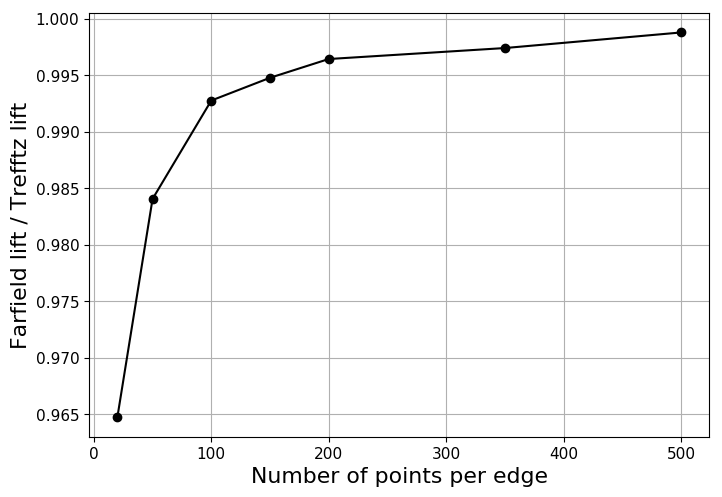
\includegraphics[width=0.49\textwidth]{images/2bbox_lift_convergence.png}}
  \subfloat[Rate of change of downward momentum]{
    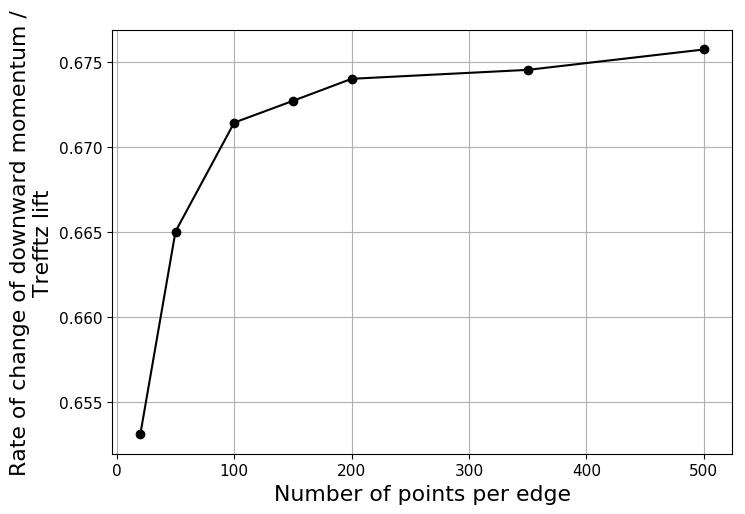
\includegraphics[width=0.49\textwidth]{images/2bbox_momrate_convergence.png}}
\caption{Grid convergence for box with side lengths $2b$.}
\label{fig:2bbox_convergence}
\end{figure}

\begin{figure}
\centering
  \subfloat[Lift]{
    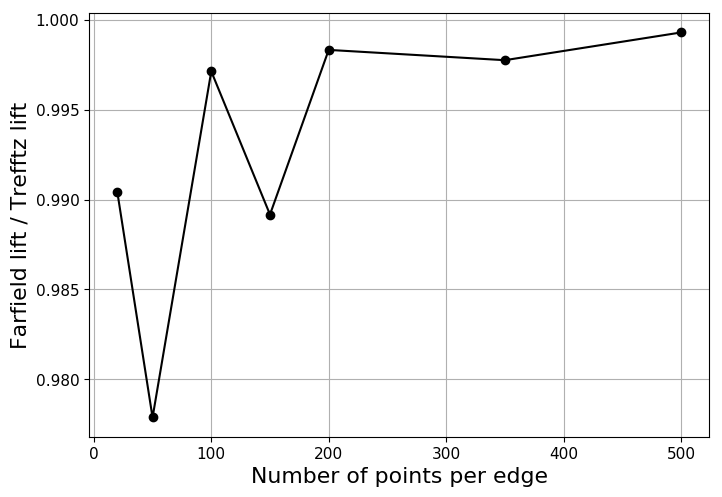
\includegraphics[width=0.49\textwidth]{images/10bbox_lift_convergence.png}}
  \subfloat[Rate of change of downward momentum]{
    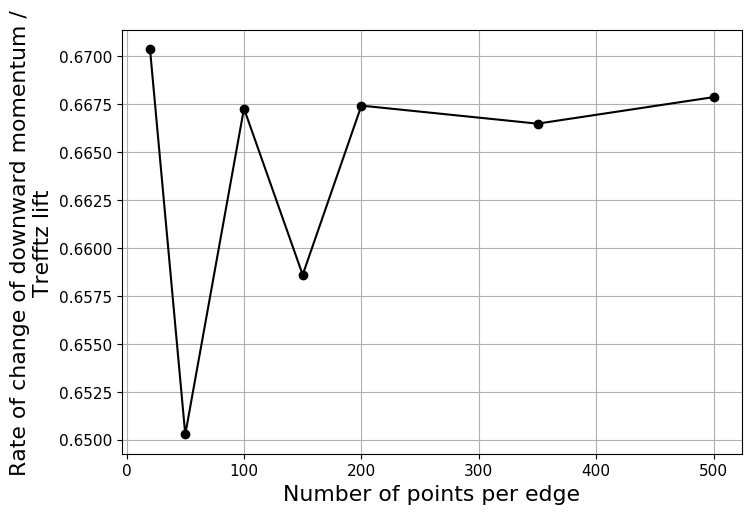
\includegraphics[width=0.49\textwidth]{images/10bbox_momrate_convergence.png}}
\caption{Grid convergence for box with side lengths $10b$.}
\label{fig:10bbox_convergence}
\end{figure}

\begin{figure}
\centering
  \subfloat[Lift]{
    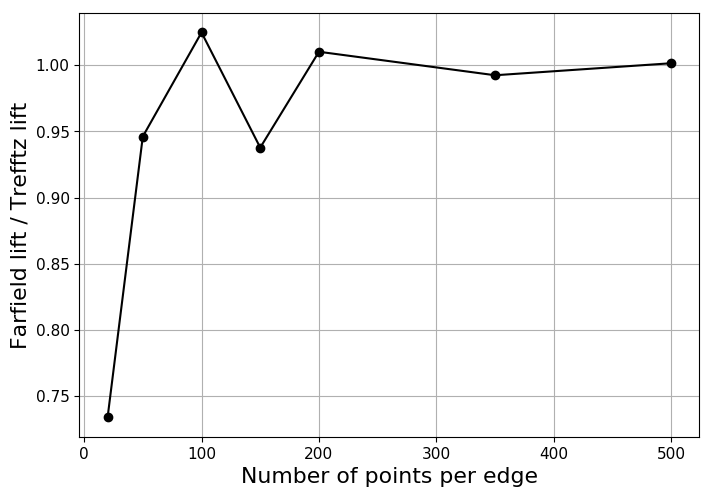
\includegraphics[width=0.49\textwidth]{images/50bbox_lift_convergence.png}}
  \subfloat[Rate of change of downward momentum]{
    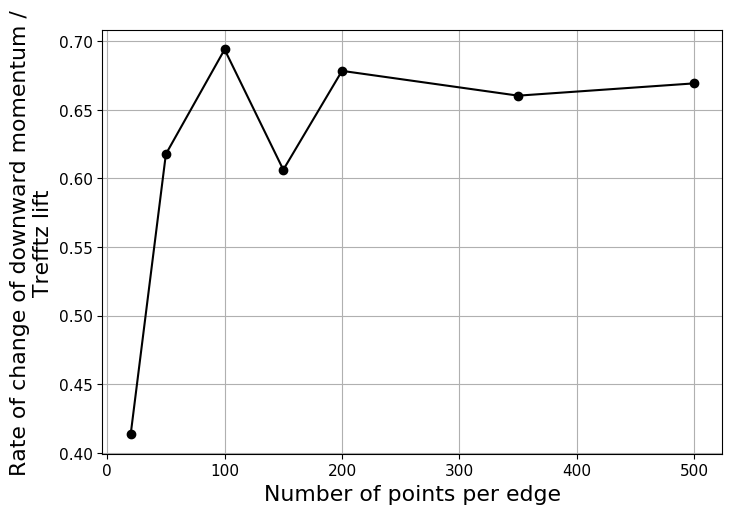
\includegraphics[width=0.49\textwidth]{images/50bbox_momrate_convergence.png}}
\caption{Grid convergence for box with side lengths $50b$.}
\label{fig:50bbox_convergence}
\end{figure}

The box with side lengths $2b$ produces a smooth, nearly-asymptotic convergence
as the number of points per edge is increased. The larger boxes produce less
smooth results
when there are fewer than 200 points per edge. This behavior is believed to be
due to poor resolution of the tip vortices on the back face of the box.
Considering that it is intended to evaluate the rate of change of downward
momentum accurately for very large boxes, the remaining calculations in this
paper use 500 points per edge to minimize discretization error. A better method
would be one that could locally refine the panels on the box as needed where
large velocity or pressure gradients are present, but for the purposes of this
paper, a fine discretization is used everywhere instead (and the large
computational cost is accepted).

\subsection{Momentum and Lift}

Observant readers will notice that for all three boxes evaluated in Section
\ref{sec:grid_convergence}, the rate of change of downward momentum in the
volume was roughly 67\% the lift. In this section, the relationship between
lift and rate of change of downward momentum is explored for many different box
sizes, with side lengths ranging from $1.01b$ to $50b$, as well as different
shapes.

\begin{figure}
\centering
  \subfloat[Cubic box]{
    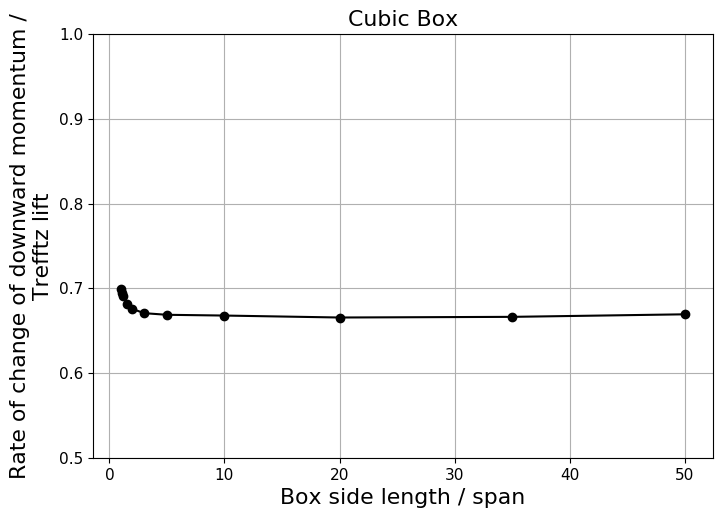
\includegraphics[width=0.49\textwidth]{images/cubic_box_momrate.png}}

  \subfloat[5:5:1 box]{
    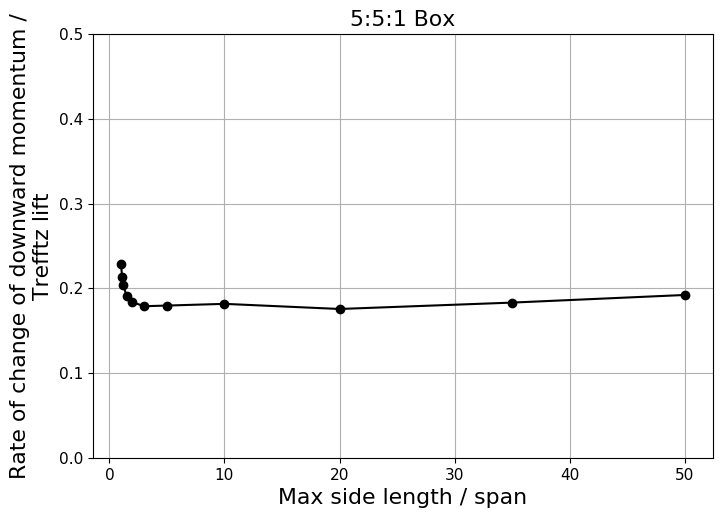
\includegraphics[width=0.49\textwidth]{images/5-5-1_box_momrate.png}}
  \subfloat[1:5:5 box]{
    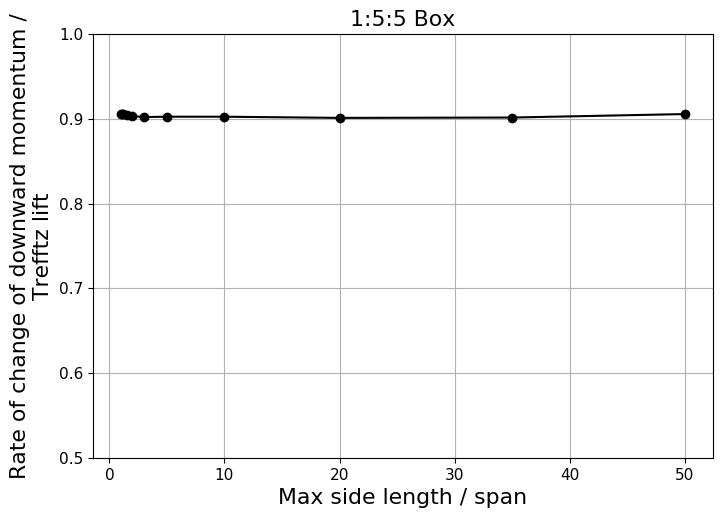
\includegraphics[width=0.49\textwidth]{images/1-5-5_box_momrate.png}}
\caption{Ratio of rate of change of downward momentum to lift for fluid domains
         of different shapes and sizes.}
\label{fig:box_momrate}
\end{figure}

Figure \ref{fig:box_momrate}a) shows the ratio of the rate of change of
downward momentum in the volume to lift as the size of the box increases, for a
cubic box. When the side length is barely larger than the wingspan, this ratio
is 0.7. The ratio decreases slightly to roughly 67\% as the side length
increases to 50 times the span. There are some small variations in the rate of
change of downward momentum between box sizes of $10b$ and $50b$, but these are
within the range of discretization error. This result makes it clear that, even
as the size of the volume of air becomes very large, the rate of change of
downward momentum does \textit{not} become equal to the lift, but rather,
some significant amount less (in this case, it is only 67\% of the lift). The
rest of the ``missing'' force is produced by pressure on the outer boundaries
of the box.

Next, two additional box shapes are considered, one with a 5:5:1 aspect ratio
(small height compared to length and span), and another with a 1:5:5 aspect
ratio (small length compared to height and span). The results are striking: the
shape of the box has a huge influence on the rate of change of momentum of the
air in the box, even as the volume of air enclosed becomes very large. For the
5:5:1 box, the rate of change of downward momentum is about 19\% the lift, while
for the 1:5:5 box, it is about 90\% the lift. These results are presented in
Fig. \ref{fig:box_momrate}(b) and (c). Despite the differing rate of change of
downward momentum, lift computed either by
Trefftz plane analysis or by Eq. \ref{eq:lift_numerical} remains the same. This
result
presents a major issue for those who support the erroneous claim that lift is
equal to the rate of change of downward momentum -- how could lift be
calculated or predicted using this method? One would have to choose the
size and shape of the fluid volume to consider and be able to guarantee that
the influence of pressure on the outer boundaries of the volume is identically
zero. It is not sufficient to just choose an arbitrary shape of large size,
because the rate of change of downward momentum is dependent on the shape.

\section{Conclusions}

\begin{itemize}
  \item Air's momentum is affected by the force applied by the aircraft as well
        as the forces (especially pressure forces) applied at the outer
        boundaries.
  \item As the volume of fluid under consideration becomes very large, the
        forces applied by the outer boundaries do not, in general, go to zero.
        Therefore, in
        general, lift is not equal to the rate of change of downward momentum of
        air influenced by the wing or aircraft.
  \item The rate of change of downward momentum depends on the shape of the
        collection of air considered. For the wing analyzed here, for a cubic
        box
        the rate of change of downward momentum was approximately 67\% the lift,
        for a 5:5:1 aspect ratio box it was approximately 19\% the lift, and for
        a 1:5:5 aspect ratio box it was approximately 90\% the lift.
\end{itemize}

\end{document}
